\documentclass{jsarticle}
\usepackage[dvipdfmx]{graphicx}
\usepackage{indentfirst}
\usepackage{multirow}
\usepackage{here}
\usepackage{listings, jlisting}

\renewcommand{\lstlistingname}{リスト}
\lstset{language=c,
  numbers=left,
  breaklines=true,
  basicstyle=\scriptsize,
  tabsize=2
}

\title{学習と進化的計算 課題レポート}
\author{C0114265 志太 悠真}

\begin{document}

\maketitle

\part{ホップフィールドネットワーク}
\section{プログラム}
\lstinputlisting[caption=Hopfield.c]{../Hopfield/Hopfield.c}

\section{解説}
\input{Hopfield}

\section{実行結果}
パターンを6番、ノイズレベルを20\%に設定して実行した結果をリスト\ref{Hopfield_result}に示す。
\lstinputlisting[caption=Hopfield.cの実行結果の例,label=Hopfield_result]{../Hopfield/output.log}

\section{考察}
パターン6(ペンギン)での入力のノイズレベルと想起の成功率の関係について検証を行なった。
想起の成功率は正解と等しいビットの割合とし、各ノイズレベルについて2000回行なった平均とした。

検証結果を図\ref{noise_success_rate}に示す。
\begin{figure}[H]
	\begin{center}
		\includegraphics[width=\hsize]{Hopfield/error.png}
		\caption{入力のノイズレベルと想起の成功率の関係\label{noise_success_rate}}
	\end{center}
\end{figure}

図\ref{noise_success_rate}から、30\%程度までのノイズの影響を受けず、40\%付近から急激にノイズの影響を受けるようになることが分かる。
今回使用した成功率の定義では成功率0\%とは期待する出力が反転したものが出力されたということであるが、ノイズレベルが70\%以上でこのような反転した出力が出るようになっている。
すなわち、ホップフィールドネットワークに1と0を反転させた入力を与えた場合、反転した出力が行なわれることが分かる。

これは、今回作成したプログラムでは一定確立でビットを反転させるという方法でノイズを乗せたため、ノイズレベル50\%の入力が最も期待する出力から離れたパターンになり、それ以上のレベルにすると期待する出力を反転したものに近づいてゆくことになったからであると考えられる。

\part{誤差逆伝播法}
\section{プログラム}
\lstinputlisting[caption=BP.c]{../BP/BP.c}

\section{解説}
\input{BP}

\section{実行結果}
上記プログラムにリスト\ref{BP_input_digital}に示すXORのパターンを入力した場合の出力結果をリスト\ref{BP_output}に示す。
\lstinputlisting[caption=使用した入力パターン,label=BP_input_digital]{../BP/xor.dat}
\lstinputlisting[caption=BP.cの実行結果の例,label=BP_output]{../BP/output.log}

また、実行時のエラーレベルの推移を図\ref{BP_error_level}に示す。
\begin{figure}[H]
	\begin{center}
		\includegraphics[width=\hsize]{../BP/error.png}
		\caption{エラーレベルの推移\label{BP_error_level}}
	\end{center}
\end{figure}

\section{考察}
作成したプログラムに対し、前掲した1か0のみのデジタル値からなる入力パターン(リスト\ref{BP_input_digital})と、入力を0から1までのアナログにしたパターン(リスト\ref{BP_input_analog})の二種類を入力し、出力のスコアを比較した。
なお、デジタル値での入力パターン数が4パターンなのに対しアナログでは100パターンと多く用意したため1回のループでの学習量がアナログの時の方が多いと考え、学習回数をデジタルで350000回に対しアナログでは3500回と設定した。
\lstinputlisting[caption=アナログ値によるXORの入力パターン(先頭10行のみ),label=BP_input_analog]{BP/analog_xor_head.dat}

上記のデジタル・アナログ二種の入力を行なった計算を100回行ないスコアの平均を計算したところ、デジタルで$0.168025$、アナログで$0.379443$となった。
アナログでの入力を行なった場合のエラーレベルの推移を図\ref{BP_analog_error}に示す。
\begin{figure}[H]
	\begin{center}
		\includegraphics[width=\hsize]{BP/analog_error.png}
		\caption{アナログで入力した場合のエラーレベルの推移\label{BP_analog_error}}
	\end{center}
\end{figure}
図\ref{BP_error_level}と図\ref{BP_analog_error}を比較すると、デジタルで入力した場合の図\ref{BP_error_level}に比べアナログで入力した場合の図\ref{BP_analog_error}の方が最大、最小ともに高く、また差も広いことが分かる。すなわち、アナログ入力の方が学習の開始時、終了時共に誤差が大きくなっている。
しかし、どちらの場合でもグラフの形状は類似しており、開始直後は学習が進まず、ある時点で急激に学習が進行し、その後変化が少なくなるという挙動は入力の特性に依らないことが分かる。

アナログでの入力・学習を行なった場合に誤差が大きくなる原因であるが、出力が0になる入力と1になる入力の境目付近の値が入力されることがあるため、これにより誤差が大きくなったものと思われる。

以上のことから、誤差逆伝播法による学習では入力値のパターンがより少なく、分割しやすい問題である方が良い結果を出すことが出来ることが分かった。


\part{自己組織化マップ}
\section{プログラム}
\lstinputlisting[caption=SOM.c]{../SOM/SOM.c}

\section{解説}
\input{SOM}

\section{実行結果}
\lstinputlisting[caption=SOM.cの実行結果の例]{../SOM/output.log}

\section{考察}
自己組織化マップにおける出力層の大きさの影響を調べるため、マップのサイズを5, 10, 20にして出力を検証した。実行結果をリスト\ref{SOM_map_5}からリスト\ref{SOM_map_15}に示す。

\lstinputlisting[caption=マップのサイズが$5\times5$のときの出力の一例, label=SOM_map_5]{SOM/map_5.txt}
\lstinputlisting[caption=マップのサイズが$10\times10$のときの出力の一例, label=SOM_map_10]{SOM/map_10.txt}
\lstinputlisting[caption=マップのサイズが$15\times15$のときの出力の一例, label=SOM_map_15]{SOM/map_15.txt}

マップのサイズ$5\times5$のときの出力であるリスト\ref{SOM_map_5}に表示された動物の種類が少ないのは、複数の動物が同じ場所に重なったからである。

マップのサイズが$10\times10$のときのリスト\ref{SOM_map_10}と、$15\times15$のときのリスト\ref{SOM_map_15}では分類の精度に大きな差は無いように見受けられる。
一方マップのサイズが$5\times5$の出力(リスト\ref{SOM_map_5})では分類には成功しているようであるが、前述の通り複数の動物が同じ場所に分類されてしまった。
この事から、検証した範囲においてはマップのサイズを大きくすることは精度に大きな影響を与えないが、入力に対して小さすぎるマップサイズを指定すると十分な分類が出来ないことが分かる。

ただし、入力を増やすことなくより大きな出力マップを計算する場合、δの値を大きくしなければ周辺の出力に対して影響を与えることが出来なくなり、精度が低下すると考えられる。
マップサイズの拡大に共なって入力を増やすのであれば隣接する出力との距離が近くなるため、δの値を大きくしなくとも分類が可能になると思われるが、一回の学習で影響を与える範囲が狭くなるため、長時間の学習が必要になると考えられる。


\part{遺伝的アルゴリズム}
\section{プログラム}
\lstinputlisting[caption=GA.c]{../GA/GA.c}

\section{解説}
\input{GA}

\section{実行結果}
\lstinputlisting[caption=GA.cの実行結果の例]{../GA/output.log}

\section{考察}
今回の実装では交叉方式として一点交叉、二点交叉、一様交叉の三種類、選択方式としてルーレット方式とトーナメント方式の二種類を実装した。
これらの方式の組み合せについて、最適解が出るまでの世代数を検証した。
検証に用いたパラメータを表\ref{GA_params}に示す。

\begin{table}[H]
	\caption{性能検証に用いたパラメータ\label{GA_params}}
	\begin{center}
		\begin{tabular}{|l|r|} \hline
			遺伝子の長さ & 100 \\ \hline
			一世代の遺伝子の数 & 40 \\ \hline
			突然変異の確率 & 1\% \\ \hline
		\end{tabular}
	\end{center}
\end{table}

検証結果を表\ref{GA_compare}および図\ref{GAor}から図\ref{GArt}に示す。

\begin{table}[H]
	\caption{交叉方式、選択方式の性能比較\label{GA_compare}}
	\begin{center}
		\begin{tabular}{|l|l|r|} \hline
			交叉方式 & 選択方式 & 最適解までの世代数 \\ \hline\hline
			一様交叉 & トーナメント & 32 \\ \hline
			二点交叉 & トーナメント & 81 \\ \hline
			一点交叉 & トーナメント & 94 \\ \hline
			二点交叉 & ルーレット & 1007 \\ \hline
			一点交叉 & ルーレット & 1434 \\ \hline
			一様交叉 & ルーレット & 6242 \\ \hline
		\end{tabular}
	\end{center}
\end{table}

\begin{figure}[H]
	\begin{tabular}{c}
		\begin{minipage}{0.5\hsize}
			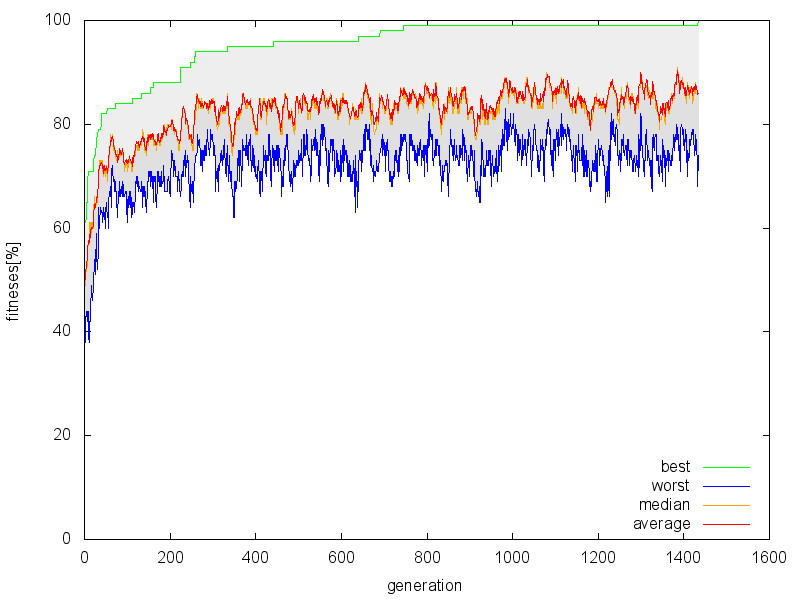
\includegraphics[width=\hsize]{GA/one-roullette.png}
			\caption{一点交叉、ルーレット方式での実行結果\label{GAor}}
		\end{minipage}

		\begin{minipage}{0.5\hsize}
			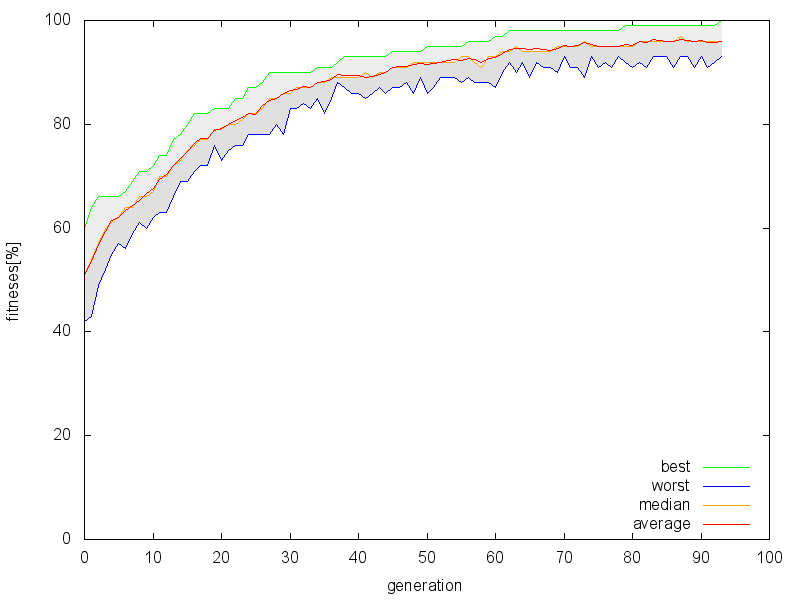
\includegraphics[width=\hsize]{GA/one-tournament.png}
			\caption{一点交叉、トーナメント方式での実行結果\label{GAot}}
		\end{minipage}
	\end{tabular}
\end{figure}

\begin{figure}[H]
	\begin{tabular}{c}
		\begin{minipage}{0.5\hsize}
			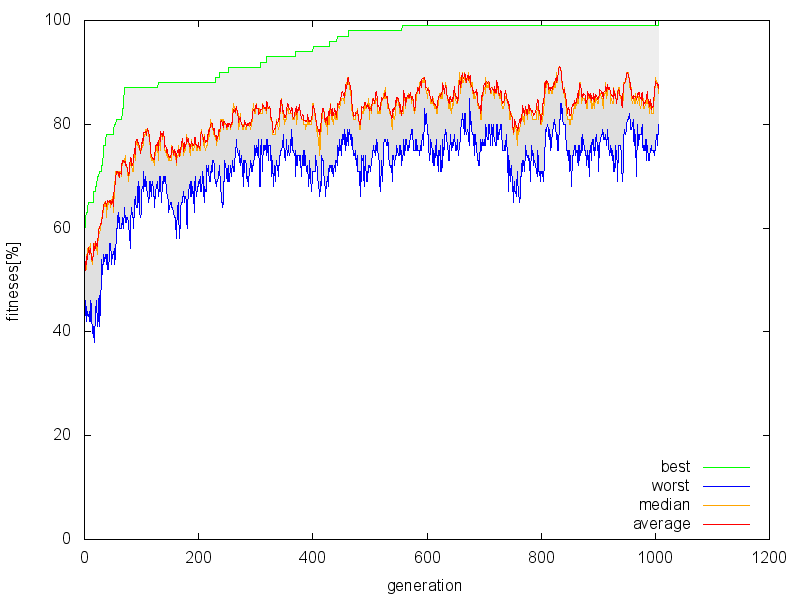
\includegraphics[width=\hsize]{GA/two-roullette.png}
			\caption{二点交叉、ルーレット方式での実行結果\label{GAtr}}
		\end{minipage}

		\begin{minipage}{0.5\hsize}
			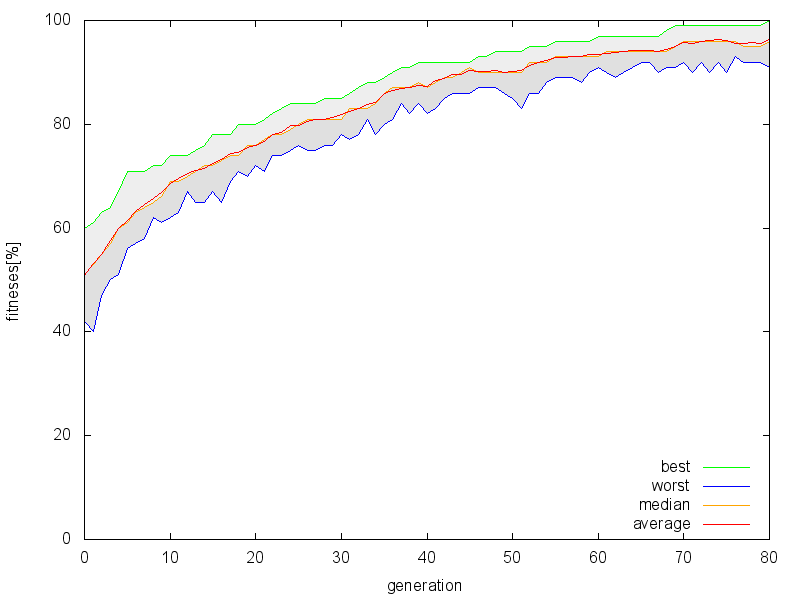
\includegraphics[width=\hsize]{GA/two-tournament.png}
			\caption{二点交叉、トーナメント方式での実行結果\label{GAtt}}
		\end{minipage}
	\end{tabular}
\end{figure}

\begin{figure}[H]
	\begin{tabular}{c}
		\begin{minipage}{0.5\hsize}
			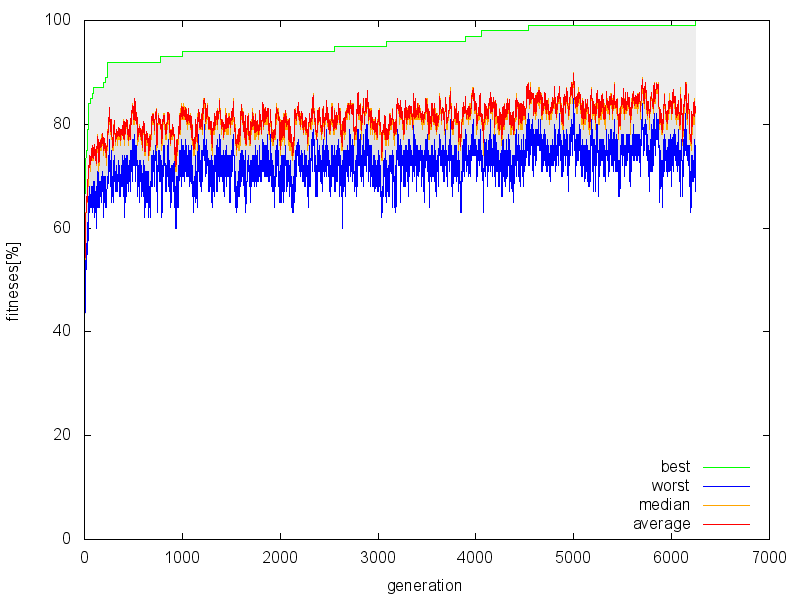
\includegraphics[width=\hsize]{GA/rand-roullette.png}
			\caption{一様交叉、ルーレット方式での実行結果\label{GArr}}
		\end{minipage}

		\begin{minipage}{0.5\hsize}
			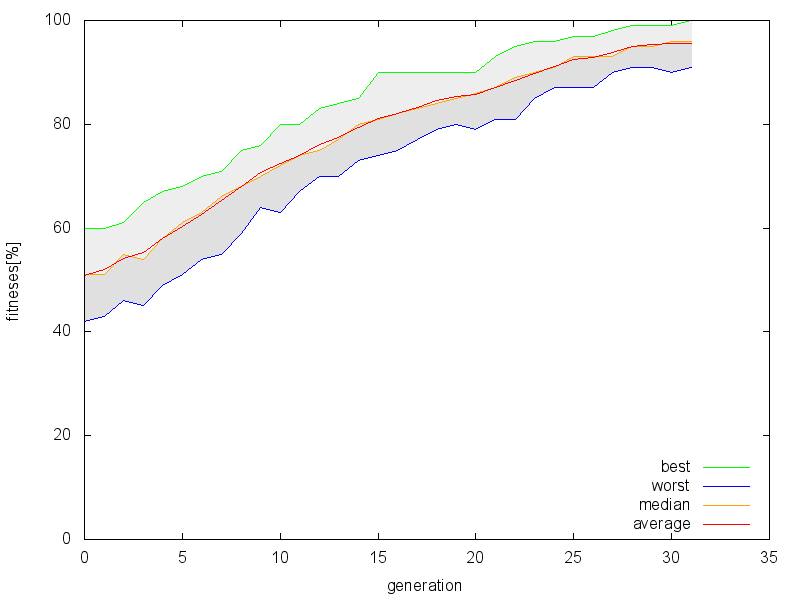
\includegraphics[width=\hsize]{GA/rand-tournament.png}
			\caption{一様交叉、トーナメント方式での実行結果\label{GArt}}
		\end{minipage}
	\end{tabular}
\end{figure}

ルーレット方式、トーナメント方式で少なくとも10倍以上の差が出ており、今回の問題ではトーナメント方式の方がより効率的であるという結果が出た。
図を見るとトーナメント方式ではルーレット方式に比べ各世代の最良値と最悪値の幅が狭く、トーナメント方式は選択圧が強いことが分かる。
本実験で用いた問題には局所解が無いことから、選択圧がより強い方がよりよい結果が出たものと考えられる。

また、ルーレット方式では最も必要な世代数が多かった一様交叉であるが、トーナメント方式では最短で最適解に至った。
一様交叉では二点交叉に比べ親の遺伝子配列を大きく崩す可能性が高いとされるが、選択圧の高いトーナメント方式ではこの特性の悪影響が出づらかったためとより良い結果が出たと考えられる。

以上のことから、問題に応じて交叉や選択の方式を変えることが非常に重要であることが分かった。

\end{document}
